\documentclass{article}
\usepackage[utf8]{inputenc}
\usepackage[portuges]{babel}
\usepackage{csquotes}
\usepackage{geometry}
\usepackage[pdftex]{hyperref}
\usepackage{indentfirst}
\usepackage{amsthm}
\usepackage{amssymb}
\usepackage{amsmath}
\usepackage{mathrsfs}
\usepackage{graphicx}
\usepackage{float}
\usepackage{multicol}
\usepackage{verbatim}
\usepackage{dsfont}
\usepackage{pgfplots}
\pgfplotsset{compat = 1.15}

\newtheorem{theorem}{Teorema}
\newtheorem{definition}{Definição}
\newtheorem{lemma}{Lema}
\newtheorem{example}{Exemplo}
\newtheorem{proposition}{Proposição}
\newtheorem{corollary}{Corolário}

\geometry{left = 3cm, top = 3cm, bottom = 2cm, right = 2cm}

\title{Geodésicas}
\author{Cristhian Grundmann \\ Igor Patrício Michels}
\date{\today}

\begin{document}

\maketitle
\section{Introdução}

Em diversas situações cotidianas a gente pode se perguntar ``qual o menor caminho de ir daqui até o supermercado?'', por exemplo. Note que a resposta nem sempre é trivial, muitas vezes ela depende de como você vai se locomover, se irá caminhando ou dirigindo, por exemplo. Nesse sentido, diversos algoritmos surgem para encontrar o menor caminho, seja em distância ou em relação ao tempo, encontrando o caminho mais rápido. Problemas similares acabam aparecendo na Teoria Local das Superfícies, buscando qual o caminho mais curto entre determinados dois pontos.

Desde a época de Euclides sabe-se que, dentro da geometria euclidiana clássica, um segmento de reta é o caminho mais curto entre dois pontos do plano. De modo simples, pode-se generalizar essa afirmação para o $\mathbb{R}^n$. Entretanto, quando estamos sobre uma superfície que não é plana, a própria noção de distância acaba sendo alterada, de forma similar a quando mudamos a geometria no plano.

Pode-se exemplificar esse fato tomando dois pontos $A$ e $B$, ambos em uma superfície $S\subset \mathbb{R}^n$. Quando definimos o segmento de reta do $\mathbb{R}^n$ que liga $A$ a $B$, não se pode afirmar que esse segmento está de fato em $S$. Ou seja, em uma superfície qualquer do $\mathbb{R}^n$, encontrar o caminho de menor distância entre dois pontos pode ser um pouco trabalhoso e, muitas vezes, contra intuitivo. Pensando nisso, o presente trabalho busca apresentar a curva de menor de distância entre dois pontos em uma determinada superfície $S\subset \mathbb{R}^n$.

\section{Motivação}

Uma das motivações para esse estudo dá pelo próprio planeta Terra. Podemos considerar a superfície terrestre como se fosse uma esfera do $\mathbb{R}^3$. Podemos ver que um segmento de reta que liga as cidades de Nova Iorque a Londres, por exemplo, não está na superfície da esfera. Além disso, ao tomarmos o caminho em ``linha reta'' entre as duas cidades, seguindo sempre à leste, por exemplo, não estaríamos minimizando a distância entre as mesmas. Pode-se ter uma melhor compreensão observando visualmente esse fato na Figura \ref{circle}.
\begin{figure}
    \centering
    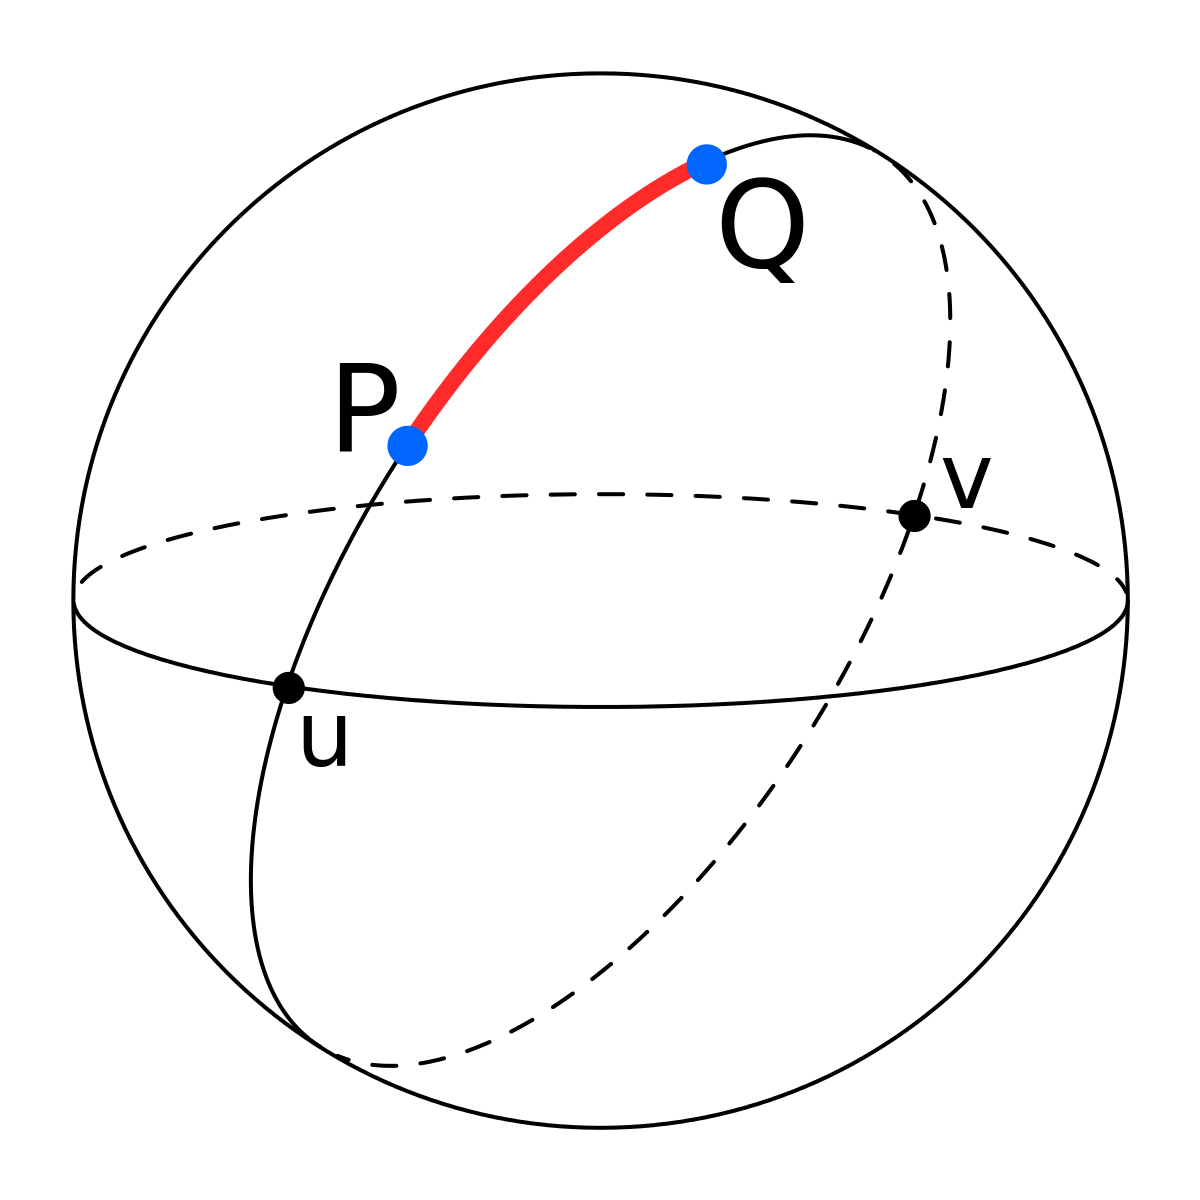
\includegraphics[scale = 0.1]{Imagens/circle.png}
    \caption{Caminho de menor distância entre os pontos $P$ e $Q$.}
    \label{circle}
\end{figure}

Note que isso tem aplicações práticas, uma das quais pode ser facilmente citada: a aviação. Em 2017 a Latam inaugurou um voo direto de Santiago, no Chile, a Melbourne, na Austrália. Visualmente, em um globo terrestre, pode-se imaginar que a melhor rota para tal viagem seria seguindo um paralelo, conforme pode-se observar na Figura \ref{pacific}. Entretanto, como o próprio piloto do voo inaugural dessa rota comentou, a rota com a menor distância se dá seguindo a direção Sul, se aproximando do Polo Sul, e então ir em rumo à Austrália, ao chegar próximo do Círculo Polar Antártico \cite{folha}.
\begin{figure}
    \centering
    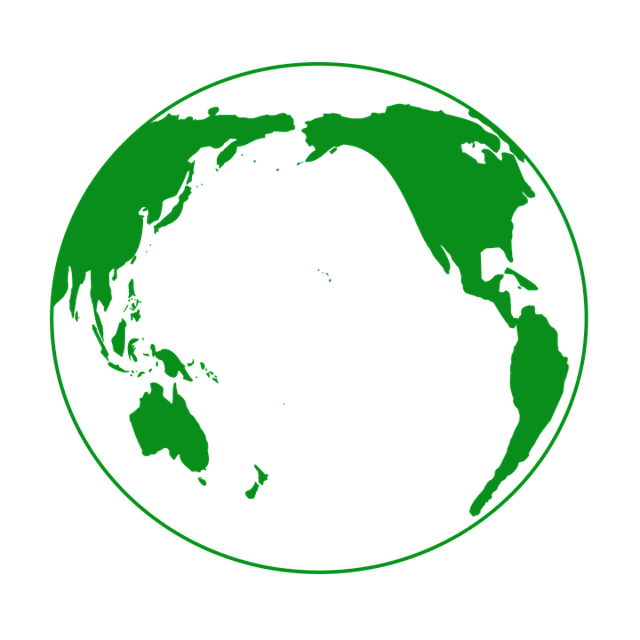
\includegraphics[scale = 0.2]{Imagens/pacific ocean.png}
    \caption{Seria um caminho paralelo ao Equador a melhor rota de ir do Chile para a Austrália?}
    \label{pacific}
\end{figure}

\section{Geodésicas}
\label{geodesicas}

Essa seção será voltada ao desenvolvimento das definições e demonstrações relacionadas as geodésicas.

\subsection{Definições e Propriedades Iniciais}

\begin{definition}
    \label{def1}
    Dada uma superfície $S\subset \mathbb{R}^3$, uma geodésica é uma curva $\alpha : I\subseteq\mathbb{R}\to S$ que representa o análogo a uma reta em um plano, isso é, uma curva que tem aceleração nula em relação à $S$.
\end{definition}

Note que ao definirmos a Aplicação Normal de Gauss em uma superfície $S$, isso é, ao definir a aplicação $N : S\to \mathbb{R}^3$, podemos reescrever a Definição \ref{def1} como segue:
\begin{definition}
    \label{def2}
    Dada uma superfície regular orientada por $N : S\to \mathbb{R}^3$, uma curva regular $\alpha : I\subseteq\mathbb{R}\to S$ é uma geodésica se $\alpha''(t)$ é perpendicular a $S$ em $\alpha(t)$ para todo ponto $t\in I$.
\end{definition}

Dessa forma, podemos interpretar as geodésicas como curvas com aceleração nula ou, equivalentemente, vetor tangente com norma constante, como visto na Proposição \ref{prop1}.
\begin{proposition}
    \label{prop1}
    Se $\alpha : I\subseteq\mathbb{R}\to S$ é uma geodésica, então $\|\alpha'(t)\|$ é constante.
\end{proposition}
\begin{proof}
    Se $\alpha$ é uma geodésica em $S$, então $\alpha''(t)$ é perpendicular a $S$ em $\alpha(t)$. Dessa forma, temos $\alpha'(t)\perp \alpha''(t)\implies \langle \alpha'(t), \alpha''(t)\rangle = 0$. Agora considere a função $\|\alpha'(t)\|^2 = \langle \alpha'(t), \alpha'(t)\rangle$. Note que
    \[\dfrac{d}{dt}\|\alpha'(t)\|^2 = \dfrac{d}{dt}\langle \alpha'(t), \alpha'(t)\rangle = 2\langle \alpha'(t), \alpha''(t)\rangle = 0,\]
    
    \noindent de onde sai que $\|\alpha'(t)\|^2$ é constante e, consequentemente, $\|\alpha'(t)\|$ é constante.
\end{proof}

Outra proposição que podemos enunciar e demonstrar é a que segue.
\begin{proposition}
    \label{prop2}
    Se $\alpha : I_1\subseteq\mathbb{R}\to S$ é uma geodésica, então sua parametrização por comprimento de arco, $\beta : I_2\subseteq\mathbb{R}\to S$, também é uma geodésica.
\end{proposition}
\begin{proof}
    Tome a função comprimento de arco $s(t) = \int_0^t \|\alpha'(t)\| ~dt$. Pela Proposição \ref{prop1}, $\|\alpha'(t)\|$ é constante, logo, $s(t) = t\|\alpha'(t)\|$. Agora sabemos que $\alpha(t) = \beta(s(t))$, dessa forma, derivando duas vezes se obtém:
    \[\alpha'(t) = \beta'(s(t))s'(t) = \beta'(s(t))\|\alpha'(t)\| \text{ e}\]
    \[\alpha''(t) = \beta''(s(t))s'(t)\|\alpha'(t)\| + \beta'(s)\left(\|\alpha'(t)\|\right)' = \beta'(s(t))\|\alpha'(t)\|^2.\]
    
    Note que isso implica que $\beta''(s(t))$ é um múltiplo de $\alpha''(t)$, logo, $\beta''(s(t))$ também é perpendicular a $S$ em $\alpha(t) = \beta(s(t))$, ou seja, $\beta$ também é uma geodésica.
\end{proof}

Agora, se $\alpha$ é uma curva de $S$, de modo que $\|\alpha'(t)\|$ é constante. Nesse caso, pode-se afirmar que o conjunto $\{T, N, T\times N\}$, com $T = T(\alpha(t)) = \alpha'(t)$ e $N = N(\alpha(t))$ é uma base ortogonal para $\mathbb{R}^3$ em todo ponto de $\alpha$. Além disso, por $\|\alpha'(t)\|$ ser constante, percebe-se que $\alpha''(t)\perp T$, ou seja, podemos escrever
\begin{equation}
    \label{eq1}
    \alpha''(t) = \kappa_n\cdot N + \kappa_g\cdot (N\times T).
\end{equation}

Dessa forma, podemos definir formalmente a curvatura normal e a curvatura geodésica:
\begin{definition}
    \label{def3}
    Dada uma superfície $S\subset \mathbb{R}^3$ e uma curva $\alpha : I\subseteq\mathbb{R}\to S$ qualquer, os valores reais $\kappa_n$ e $\kappa_g$ que satisfazem a Equação \ref{eq1} são chamados, respectivamente, \textbf{Curvatura Normal} e \textbf{Curvatura Geodésica} de $\alpha$ no ponto $t$.
\end{definition}

Note que utilizando as Definições \ref{def2} e \ref{def3}, podemos enunciar uma nova definição de geodésica.
\begin{definition}
    \label{def4}
    Dada uma superfície $S\subset \mathbb{R}^3$ e uma curva $\alpha : I\subseteq\mathbb{R}\to S$, $\alpha$ é uma geodésica em $S$ se $\kappa_g$ é nula para todo ponto de $\alpha$.
\end{definition}

Tendo tais definições feitas, podemos partir para o teorema que vai nos possibilitar dizer se uma curva é ou não uma geodésica.

\subsection{Caracterizando uma Geodésica}

\begin{theorem}
    \label{teo1}
    Seja $S$ uma superfície regular. Seja também $X : D\subseteq \mathbb{R}^2\to S$, com a primeira forma fundamental de $X$ igual a $Edu^2 + 2Fdudv + Gdv^2$, e tome a curva regular $\alpha : I\subseteq\mathbb{R}\to S$ de modo que $\alpha(t) = X(u(t), v(t))$. Temos que $\alpha$ é uma geodésica se, e somente se, o seguinte sistema de equações é satisfeito:
    \begin{equation}
        \label{eq_geo}
        \left\{\begin{array}{cc}
            \dfrac{d}{dt}(Eu' + Fv') & = \dfrac{1}{2}(E_u (u')^2 + 2F_u u'v' + G_u (u')^2) \vspace{6pt}\\
            \dfrac{d}{dt}(Fu' + Gv') & = \dfrac{1}{2}(E_v (u')^2 + 2F_v u'v' + G_v (u')^2)
        \end{array}\right..
    \end{equation}
    
    As Equações de \ref{eq_geo} são chamadas de \textbf{Equações Geodésicas}.
\end{theorem}
\begin{proof}
    Sabendo que $\{X_u, X_v\}$ é a base do plano tangente que é tangente a $S$ em $\alpha(t)$, então $\alpha$ será geodésica se, e somente se, $\alpha''$ é perpendicular a $X_u$ e a $X_v$. Como $\alpha' = u' X_u + v' X_v$, essa relação se resume a
    \begin{equation}
        \label{rest}
        \left\{\begin{array}{cc}
            \left\langle \dfrac{d}{dt}(u' X_u + v' X_v), X_u\right\rangle & = 0 \vspace{6pt}\\
            \left\langle \dfrac{d}{dt}(u' X_u + v' X_v), X_v\right\rangle & = 0
        \end{array}\right..
    \end{equation}
    
    Note que
    \begin{align*}
        \left\langle \dfrac{d}{dt}(u' X_u + v' X_v), X_u\right\rangle & = \dfrac{d}{dt}\langle u' X_u + v' X_v, X_u\rangle - \left\langle u' X_u + v' X_v, \dfrac{d}{dt}X_u\right\rangle \\
        & = \dfrac{d}{dt}(Eu' + Fv') - \langle u' X_u + v' X_v, u' X_{uu} + v' X_{uv}\rangle \\
        & = \dfrac{d}{dt}(Eu' + Fv') - (u')^2\langle X_u, X_{uu}\rangle - u'v'(\langle X_u, X_{uv}\rangle + \langle X_v, X_{uu}\rangle) - (v')^2\langle X_v, X_{uv}\rangle
    \end{align*}
    
    Agora, veja que
    \[E_u = \langle X_u, X_u\rangle_u = \langle X_{uu}, X_u\rangle + \langle X_u, X_{uu}\rangle = 2\langle X_u, X_{uu}\rangle\]
    \[G_u = \langle X_v, X_v\rangle_u = \langle X_{vu}, X_v\rangle + \langle X_v, X_{vu}\rangle = 2\langle X_v, X_{vu}\rangle\]
    
    \noindent ou seja, temos que $\langle X_u, X_{uu}\rangle = \frac{1}{2}E_u$ e $\langle X_v, X_{uv}\rangle = \frac{1}{2}G_u$. Note também que
    \[\langle X_u, X_{uv}\rangle + \langle X_v, X_{uu}\rangle = \langle X_u, X_v\rangle_u = F_u.\]
    
    Perceba que, com isso, podemos substituir os produtos escalares encontrados no desenvolvimento da primeira equação. Dessa forma
    \begin{align*}
        \left\langle \dfrac{d}{dt}(u' X_u + v' X_v), X_u\right\rangle & = \dfrac{d}{dt}(Eu' + Fv') - \dfrac{1}{2}(u')^2E_u - u'v'F_u - \dfrac{1}{2}(v')^2G_u \\
        & = \dfrac{d}{dt}(Eu' + Fv') - \dfrac{1}{2}\left((u')^2E_u + 2u'v'F_u + (v')^2G_u\right)
    \end{align*}
    
    Note que isso mostra que a primeira equação do Sistema de Equações \ref{rest} é equivalente a primeira equação do Sistema de Equações \ref{eq_geo}. De modo análogo, mostra-se a equivalência da segunda equação do Sistema de Equações \ref{rest} com a segunda equação do Sistema de Equações \ref{eq_geo}.
\end{proof}

Note que as Equações Geodésicas vistas no Teorema \ref{teo1} definem um sistema de EDO's de ordem 2, o que nos leva ao seguinte teorema.
\begin{theorem}
    \label{teo2}
    Seja $S$ uma superfície regular e $p$ um ponto de $S$. Seja também $v\in T_pS$, então existe apenas uma geodésica $\alpha$ em $S$ de modo que $\alpha(0) = p$ e $\alpha'(0) = v$. Alternativamente, podemos dizer que existe apenas uma geodésica que passa por $p$ com velocidade $v$.
\end{theorem}
\begin{proof}
    A demonstração para esse teorema sai diretamente ao aplicar o Teorema de Existência e Unicidade de EDO's de um sistema com condição inicial.
\end{proof}

Tendo em mãos esse resultado, podemos definir a geodésica resultante como segue.
\begin{definition}
    \label{def5}
    A geodésica $\alpha$ em $S$ que satisfaz as condições dadas no Teorema \ref{teo2} será denotada por $\alpha_{p, v}$ e será definida no intervalo real $(-\varepsilon, \varepsilon)$, de modo que esse seja o maior intervalo simétrico onde tal geodésica é definida.
\end{definition}

Dessa forma, podemos tomar $\lambda > 0$ e definir uma nova curva $\beta$ de modo que
\begin{align*}
    \beta : \left(-\dfrac{\varepsilon}{\lambda}, \dfrac{\varepsilon}{\lambda}\right) & \to S \\
    t & \mapsto \alpha_{p, v}(\lambda t).
\end{align*}

Vemos facilmente que $\beta$ é geodésica, pois $\beta''(t) = \lambda^2\alpha_{p, v}(\lambda t)$ é perpendicular a $S$ no ponto $\beta(t) = \alpha_{p, v}(\lambda t)$, uma vez que $\alpha_{p, v}$ é. Além disso, temos que $\beta(0) = \alpha_{p, v}(0) = p$ e $\beta'(0) = \lambda\alpha_{p, v}'(0) = \lambda v$. Assim, utilizando o resultado do Teorema \ref{teo2}, vemos que $\beta$ é a única geodésica que passa por $p$ com velocidade $\lambda v$, logo, $\beta = \alpha_{p, \lambda v}$. Esse resultado pode ser enunciado como uma proposição.
\begin{proposition}
    \label{prop3}
    Dada uma geodésica $\alpha_{p, v}$ em $S$ e $\lambda > 0$, tem-se que
    \[\forall t\in \left(-\dfrac{\varepsilon}{\lambda}, \dfrac{\varepsilon}{\lambda}\right), \alpha_{p, \lambda v}(t) = \alpha_{p, v}(\lambda t).\]
\end{proposition}
\begin{proof}
    Demonstrado acima.
\end{proof}

Uma ideia intuitiva dessa proposição é que podemos deixar o intervalo de definição de $\alpha_{p, v}$ grande à medida com que diminuímos $\|v\|$, isso é, $\alpha_{p, v}$ está definida no intervalo $(-\varepsilon, \varepsilon)$ com velocidade $\|v\|$, já $\alpha_{p, \frac{v}{n}}$ está definida no intervalo $\left(-n\varepsilon, n\varepsilon\right)$ com velocidade $\frac{1}{n}\|v\|$. Note que isso nos leva ao seguinte corolário da Proposição \ref{prop3}:
\begin{corollary}
    \label{cor1}
    Se $0 < \lambda < \varepsilon$, então a geodésica $\alpha_{p, \lambda v} : \left(-\frac{\varepsilon}{\lambda}, \frac{\varepsilon}{\lambda}\right)$ está definida para $t = 1$.
\end{corollary}

%%%%%%%%%%%%%%%%%%%%%%%%%%%%%%%%%%%%%%%%%%%%%%%%%%%%%%%%%%%%%%%%%%%%%%%%%%%%%%%%%%%%%%%%%%%%%%%%%%%%%%%%%%%%%%%%%%%%%%%%

% Podemos então introduzir uma nova definição a fim de auxiliar nas demonstrações que se seguem.
% \begin{definition}
%     \label{def6}
%     Dado um ponto $p\in S$, a bola aberta centrada em $x$ com raio $r$ e que está contida em $T_pS$ será denotada por $B(x, r)$.
% \end{definition}

% Dessa forma, podemos enunciar outra proposição que nos auxiliará mais adiante.
% \begin{proposition}
%     \label{prop4}
%     Dada uma superfície $S$ e um ponto $p\in S$, existe $\delta > 0$ de modo que se $v\in T_pS$, tal que $\|v\| < \delta$, então $\alpha_{p, v}$ está definida quando $t = 1$.
% \end{proposition}
% \begin{proof}
%     Note que pelo Corolário \ref{cor1}, para todo vetor $v$ em $T_pS$ é possível encontrar $\lambda$ de modo que $\alpha_{p, \lambda v}$ está definida em $t = 1$. Em particular, podemos tomar apenas os vetores $v$ de norma $1$, assim tomando um $\delta$ menor que o ínfimo dos respectivos $\lambda$'s temos que todos os vetores de $B(0, \delta)$ são tais que sua velocidade é menor que $\delta$ e, consequentemente, menor que $\lambda$, logo, temos que o intervalo de definição dessas geodésicas devem ser maiores que os intervalos da forma $\left(-\frac{\varepsilon}{\lambda}, \frac{\varepsilon}{\lambda}\right)$, os quais contém o $1$. Logo, temos que todo vetor $v\in T_pS$ com $\|v\| < \delta$ é tal que $\alpha_{p, v}$ está definida em $t = 1$.
% \end{proof}

% \subsection{Propriedades de Caminho Mínimo}

% Anteriormente definimos uma geodésica e apresentamos algumas propriedades básicas dessa família de curvas. Nessa seção iremos focar na demonstração da propriedade que as geodésicas possuem de minimizar localmente as distâncias em uma superfície. Para tanto, precisamos introduzir a Aplicação Exponencial.

% \subsubsection{Aplicação Exponencial}

% Utilizando o resultado da Proposição \ref{prop4}, podemos ver que, dado um ponto $p\in S$, cada um dos vetores $v\in B(0, \delta)$ é tal que $\alpha_{p, v}$ está definido para $t = 1$, onde $\alpha_{p, v}$ é como na Definição \ref{def5}. Dessa forma, podemos definir a Aplicação Exponencial.
% \begin{definition}
%     \label{def7}
%     Dado $p\in S$, uma superfície regular, definimos a Aplicação Exponencial em $p$ por
%     \begin{align*}
%         \exp_p : B(0, \delta) & \to S \\
%         v & \mapsto \alpha_{p, v}(1).
%     \end{align*}
% \end{definition}

% Perceba que, pela dependência suave das condições iniciais de um sistema de EDO's para sua solução, decorre que a função $\exp_p$ é suave, e mais ainda, diferenciável. Perceba que essa aplicação pode ser vista como difeomorfismo local.
% \begin{proposition}
%     \label{prop5}
%     Para cada ponto $p\in S$, uma superfície regular, existe $\delta > 0$ tal que a aplicação exponencial $\exp_p : B(0, \delta)\to S$ é um difeomorfismo sobre sua imagem em $S$. 
% \end{proposition}
% \begin{proof}
%     Veja página 109 de \cite{lima}.
% \end{proof}

% Note que dada uma superfície regular $S$, a Proposição \ref{prop5} nos diz que toda bola regular $B(p, \delta)\subset S$, tida como resultado da exponencial em $p$ de $B(0, \delta)$ é uma vizinhança parametrizada de $S$. Assim, juntando com o fato de que $T_pS$ é bidimensional, podemos encontrar um isomorfismo linear $A : \mathbb{R}^2\to T_pS$. Tomando $U = A^{-1}(B(0, \delta))$ temos que, uma vez que $B(0, \delta)$ é aberta, $U$ também é, logo, $X = \exp_p(B(0, \delta)\circ A)|_U$ é uma composição de difeomorfismos que leva $U$ a $B(p, \delta)$, o que mostra que $X$ é parametrização local de $S$. Com uma ideia semelhante, pode-se definir uma parametrização local de $S$ em coordenadas polares. Para isso, podemos definir as coordenadas polares em função de $(r, \theta)$ de modo que, para todo vetor $v\in T_pS\setminus \{0\}$, temos $r = \|v\|$, $\cos{\theta} = \left\langle\frac{v}{\|v\|}, v_1\right\rangle$ e $\sin{\theta} = \left\langle\frac{v}{\|v\|}, v_2\right\rangle$, onde $\{v_1, v_2\}$ é uma base ortonormal de $T_pS$ e que representará a base dessa parametrização com coordenadas polares.

% Note que a elaboração de um sistema de coordenadas polares nos possibilita escrever $v = r\nu(\theta)$, onde $\nu(\theta) = v_1\cos{\theta} + v_2\sin{\theta}$.

% Agora tomamos $\delta > 0$ de modo que a aplicação exponencial $\exp_p : B(0, \delta)\to S$ seja um difeomorfismo sobre a sua imagem $\exp_p(B(0, \delta))$. Dessa forma, podemos tomar $U = (0, \delta)\times (0, 2\pi)$ e definimos a aplicação
% \begin{align*}
%     X : U & \to S \\
%     (r, \theta) & \mapsto \exp_p(r\nu(\theta)).
% \end{align*}

% Note que novamente vale o argumento de que $X$ é uma composição de difeomorfismos, que leva um domínio de $\mathbb{R}^2$ a $S$, logo, $X$ é uma parametrização local de $S$, dita parametrização por coordenadas polares.

%%%%%%%%%%%%%%%%%%%%%%%%%%%%%%%%%%%%%%%%%%%%%%%%%%%%%%%%%%%%%%%%%%%%%%%%%%%%%%%%%%%%%%%%%%%%%%%%%%%%%%%%%%%%%%%%%%%%%%%%

\subsection{Propriedade do Caminho Mínimo}

Nas seções anteriores foram definidas e provadas algumas propriedades gerais de uma geodésica. Nessa seção iremos dar ênfase a propriedade de que a geodésica é a curva que gera o caminho mais curto entre dois pontos em uma superfície. Para isso, vamos apresentar uma solução pelo método de Euler-Lagrange.

Seja $\alpha : \mathbb{R} \to \mathbb{R}^2$ uma curva parametrizada numa carta local da superfície com forma fundamental $Edu^2 + 2Fdudv + Gdv^2$. Queremos saber se essa curva minimiza comprimento entre dois pontos, com parâmetros $a$ e $b$. O comprimento pode ser expresso pela integral
\[\int_{a}^{b} \|\alpha'(t)\|_{\alpha(t)} dt\]

usando a primeira forma fundamental no ponto $\alpha(t)$ para achar o comprimento do vetor tangente $\alpha'(t)$. Dessa forma, o integrando dessa integral é uma função que depende do ponto $\alpha(t)$ e do vetor tangente $\alpha'(t)$. Assim, podemos generalizar o problema de otimização, fazendo a otimização da integral
\[\mathcal{L}(\alpha) = \int_{a}^{b} L(\alpha(t), \alpha'(t)) dt.\]

Para isso. basta definir uma função $L : \mathbb{R}^2 \times \mathbb{R}^2 \to \mathbb{R}$.

Para caracterizar uma curva que otimiza ``localmente'' a medida dada pela função $L$, com extremos $\alpha(a)$ e $\alpha(b)$ fixos, vamos analisar perturbações suaves da curva. Para isso, supomos uma curva suave $\mu : \mathbb{R} \to \mathbb{R}^2$, onde $\mu(a) = \mu(b) = 0$. Usando um $\varepsilon > 0$ real como grau de perturbação, a curva perturbada é dada por $(\alpha + \varepsilon \mu)(t) = \alpha(t) + \varepsilon \mu(t)$. Essa curva tem extremos iguais a original. bem como parâmetros iguais.

A curva é otimizada localmente exatamente quando $\frac{d}{d\varepsilon}\mathcal{L}(\alpha + \varepsilon \mu)  \mid_{\varepsilon = 0} = 0$.
\begin{align*}
    \frac{d}{d\varepsilon} \int_{a}^{b} L(\alpha(t) + \varepsilon \mu (t), \alpha'(t) + \varepsilon \mu'(t)) dt & = \int_{a}^{b} \frac{d}{d\varepsilon} L(\alpha(t) + \varepsilon \mu (t), \alpha'(t) + \varepsilon \mu'(t)) dt \\
    & = ~~~~ \int_{a}^{b} L_u(\alpha(t) + \varepsilon \mu (t), \alpha'(t) + \varepsilon \mu'(t))\mu(t) dt \\
    & ~~~~ + \int_{a}^{b} L_v(\alpha(t) + \varepsilon \mu (t), \alpha'(t) + \varepsilon \mu'(t))\mu'(t) dt.
\end{align*}

Vamos calcular essa derivada em $\varepsilon = 0$ de modo a minimizar a função, ou seja, igualando a zero. Dessa forma, temos
\[\int_{a}^{b} L_u(\alpha(t), \alpha'(t))\mu(t) dt + \int_{a}^{b} L_v(\alpha(t), \alpha'(t))\mu'(t) dt = 0.\]

A integral indefinida do segundo termo pode ser reescrita, pela regra do produto, como
\[\int L_v(\alpha(t), \alpha'(t))\mu'(t) dt = L_v(\alpha(t), \alpha'(t))\mu(t) - \int \frac{d}{dt}L_v(\alpha(t), \alpha'(t))\mu(t)dt.\]

Note que a primeira parcela é nula, pois $\mu(a) = \mu(b) = 0$, logo, essa segunda integral se resume a
\[\int_{a}^{b} -\frac{d}{dt}L_v(\alpha(t), \alpha'(t))\mu(t)dt.\]

Então podemos reescrever a integral como
\begin{align*}
    \int_{a}^{b} L_u(\alpha(t), \alpha'(t))\mu(t) dt + \int_{a}^{b} - \frac{d}{dt}L_v(\alpha(t), \alpha'(t))\mu(t) dt & = 0 \\
    \int_{a}^{b} \left(L_u(\alpha(t), \alpha'(t)) - \frac{d}{dt}L_v(\alpha(t), \alpha'(t))\right)\mu(t)dt & = 0.
\end{align*}

Como isso vale para toda função $\mu$, devemos ter que
\[L_u(\alpha(t), \alpha'(t)) - \frac{d}{dt}L_v(\alpha(t), \alpha'(t)) = 0\]

Sabemos que a função $L$ desejada é na forma $\sqrt{f(\alpha(t), \alpha'(t))}$. Com isso, aplicando a regra da cadeia, temos
\begin{align*}
    \frac{f_u(\alpha(t), \alpha'(t))}{2\sqrt{f(\alpha(t), \alpha'(t))}} - \frac{\frac{d}{dt}f_v(\alpha(t), \alpha'(t))}{2\sqrt{f(\alpha(t), \alpha'(t))}} & = 0 \\
    f_u(\alpha(t), \alpha'(t)) - \frac{d}{dt}f_v(\alpha(t), \alpha'(t)) & = 0.
\end{align*}

Agora podemos definir $\alpha(t) = (u(t), v(t))$ e $\alpha'(t) = (u'(t), v'(t))$. Logo, podemos reescrever a função $L$, já transformando a mesma para a expressão com a forma fundamental. Assim, vale que
\[L(\alpha(t), \alpha'(t)) = L((u, v), (u', v')) = E(u, v)(u')^2 + 2F(u, v)u'v' + G(u, v)(v')^2.\]

Note que podemos reescrever a equação acima como o seguinte sistema de equações
\begin{equation*}
    \left\{\begin{array}{cc}
        E_u(u, v)(u')^2 + 2F_u(u, v)u'v' + G_u(u, v)(v')^2 & = \dfrac{d}{dt}(2E(u, v)u' + 2F(u, v)v') \vspace{6pt}\\
        E_v(u, v)(u')^2 + 2F_v(u, v)u'v' + G_v(u, v)(v')^2 & = \dfrac{d}{dt}(2F(u, v)u' + 2G(u, v)v')
    \end{array}\right..
\end{equation*}

Mas perceba que o coeficiente $2$ é constante, então ele pode sair da derivada do lado direito, o que nos possibilita reescrever o sistema acima como
\begin{equation*}
    \left\{\begin{array}{cc}
        \dfrac{1}{2}\left(E_u(u, v)(u')^2 + 2F_u(u, v)u'v' + G_u(u, v)(v')^2\right) & = \dfrac{d}{dt}(E(u, v)u' + F(u, v)v') \vspace{6pt}\\
        \dfrac{1}{2}\left(E_v(u, v)(u')^2 + 2F_v(u, v)u'v' + G_v(u, v)(v')^2\right) & = \dfrac{d}{dt}(F(u, v)u' + G(u, v)v')
    \end{array}\right..
\end{equation*}

% Derivando o lado direito das equações acima, temos
% \begin{equation*}
%     \left\{\begin{array}{cc}
%         E_u(u, v)(u')^2 + G_u(u, v)(v')^2 & = 2(E_u(u, v)(u')^2 + E_v(u, v)u'v' + E(u, v)u'') \vspace{6pt}\\
%         E_v(u, v)(u')^2 + G_v(u, v)(v')^2 & = 2(G_u(u, v)u'v' + G_v(u, v)(v')^2 + G(u, v)v'')
%     \end{array}\right..
% \end{equation*}

% Simplificando a expressão, temos
% \begin{equation}
%     \label{eq5}
%     \left\{\begin{array}{cc}
%         G_u(u, v)(v')^2 & = E_u(u, v)(u')^2 + 2E_v(u, v)u'v' + 2E(u, v)u'' \vspace{6pt}\\
%         E_v(u, v)(u')^2 & = 2G_u(u, v)u'v' + G_v(u, v)(v')^2 + 2G(u, v)v''
%     \end{array}\right..
% \end{equation}

% Note que podemos reescrever a Equação \ref{eq5} como
% \begin{equation*}
%     \left\{\begin{array}{cc}
%         u'' + \dfrac{E_u(u, v)}{2E(u, v)}(u')^2 + \dfrac{E_v(u, v)}{E(u, v)}u'v' - \dfrac{G_u(u, v)}{2E(u, v)}(v')^2 & = 0 \vspace{6pt}\\
%         v'' - \dfrac{E_v(u, v)}{2G(u, v)}(u')^2 + \dfrac{G_u(u, v)}{G(u, v)}u'v' + \dfrac{G_v(u, v)}{2G(u, v)}(v')^2 & = 0
%     \end{array}\right..
% \end{equation*}

Omitindo $(u, v)$ com o intuito de deixar a equação mais limpa, obtemos a seguinte expressão
\begin{equation}
    \label{eq6}
    \left\{\begin{array}{cc}
        \dfrac{1}{2}\left(E_u(u')^2 + 2F_uu'v' + G_u(v')^2\right) & = \dfrac{d}{dt}(Eu' + Fv') \vspace{6pt}\\
        \dfrac{1}{2}\left(E_v(u')^2 + 2F_vu'v' + G_v(v')^2\right) & = \dfrac{d}{dt}(Fu' + Gv')
    \end{array}\right..
\end{equation}

Note que a curva que minimiza a distância de $\alpha(a)$ a $\alpha(b)$ deve satisfazer o Sistema de Equações \ref{eq6}. Mas esse sistema é igual ao Sistema de Equações \ref{eq_geo}, logo, essa curva deve ser uma geodésica, ou seja, a curva que minimiza a distância de $\alpha(a)$ a $\alpha(b)$ é justamente a geodésica que passa por esses dois pontos.

%%%%%%%%%%%%%%%%%%%%%%%%%%%%%%%%%%%%%%%%%%%%%%%%%%%%%%%%%%%%%%%%%%%%%%%%%%%%%%%%%%%%%%%%%%%%%%%%%%%%%%%%%%%%%%%%%%%%%%%%

% \section{Solução por Euler-Lagrange}

% Seja $\gamma : \mathbb{R} \rightarrow \mathbb{R}^2$ uma curva parametrizada numa carta local da superfície. Queremos saber se essa curva minimiza comprimento entre dois pontos, com parâmetros $\alpha$ e $\beta$. O comprimento pode ser expresso pela integral

% \[\int_{\alpha}^{\beta} |\gamma'(t)|_{\gamma(t)} dt\]
% usando a primeira forma fundamental no ponto $\gamma$ para achar o comprimento do vetor tangente $\gamma'$.

% O integrando dessa integral é uma função que depende do ponto $\gamma$ e do vetor tangente $\gamma'$. Podemos generalizar o problema de otimização, fazendo a otimização da integral
% \[\mathcal{L}(\gamma) = \int_{\alpha}^{\beta} L(\gamma(t), \gamma'(t)) dt\]
% Basta definir uma função $L : \mathbb{R}^2 \times \mathbb{R}^2 \rightarrow \mathbb{R}$.

% Para caracterizar uma curva que otimiza ``localmente" a medida dada pela função $L$, com extremos $\gamma(\alpha)$ e $\gamma(\beta)$ fixos, vamos analisar perturbações suaves da curva. Para isso, supomos uma curva suave $\mu : \mathbb{R} \rightarrow \mathbb{R}^2$, onde $\mu(\alpha) = \mu(\beta) = 0$. Usando um $\varepsilon > 0$ real como grau de perturbação, a curva perturbada é dada por $\gamma + \varepsilon \mu$. Mais precisamente, $(\gamma + \varepsilon \mu)(t) = \gamma(t) + \varepsilon \mu(t)$. Essa curva tem extremos iguais a original e em parâmetros iguais.

% A curva é otimizada localmente exatamente quando $\frac{d}{d\varepsilon}\mathcal{L}(\gamma + \varepsilon \mu)  \mid_{\varepsilon=0} = 0$.

% \[\frac{d}{d\varepsilon} \int_{\alpha}^{\beta} L(\gamma(t) + \varepsilon \mu (t), \gamma'(t) + \varepsilon \mu'(t)) dt =\]
% \[\int_{\alpha}^{\beta} \frac{d}{d\varepsilon} L(\gamma(t) + \varepsilon \mu (t), \gamma'(t) + \varepsilon \mu'(t)) dt =\]
% \[\int_{\alpha}^{\beta} L_1(\gamma(t) + \varepsilon \mu (t), \gamma'(t) + \varepsilon \mu'(t))\mu(t) + L_2(\gamma(t) + \varepsilon \mu (t), \gamma'(t) + \varepsilon \mu'(t))\mu'(t) dt\]

% Vamos calcular essa derivada em $\varepsilon=0$. Temos
% \[\int_{\alpha}^{\beta} L_1(\gamma(t), \gamma'(t))\mu(t) + L_2(\gamma(t), \gamma'(t))\mu'(t) dt = 0\]

% A integral indefinida do segundo termo pode ser reescrita pela regra do produto como
% \[\int L_2(\gamma(t), \gamma'(t))\mu'(t) dt = L_2(\cdots)\mu(t) - \int \frac{d}{dt}L_2(\gamma(t), \gamma'(t))\mu(t)dt\]

% A integral definida dessa parte é apenas \[\int_{\alpha}^{\beta} -\frac{d}{dt}L_2(\gamma(t), \gamma'(t))\mu(t)dt\]
% pois $\mu(\alpha) = \mu(\beta) = 0$.

% A integral completa então é
% \[\int_{\alpha}^{\beta} L_1(\gamma(t), \gamma'(t))\mu(t) - \frac{d}{dt}L_2(\gamma(t), \gamma'(t))\mu(t)dt = 0\]
% \[\int_{\alpha}^{\beta} \left(L_1(\gamma(t), \gamma'(t)) - \frac{d}{dt}L_2(\gamma(t), \gamma'(t))\right)\mu(t)dt = 0\]
% Como isso vale para toda função $\mu$, temos que \[L_1(\gamma(t), \gamma'(t)) - \frac{d}{dt}L_2(\gamma(t), \gamma'(t)) = 0\]

% Sabemos que a função $L$ desejada é na forma $\sqrt{f(\gamma(t), \gamma'(t))}$. Aplicando a regra da cadeia, temos
% \[\frac{f_1(\gamma(t), \gamma'(t))}{2\sqrt{f(\gamma(t), \gamma'(t))}} - \frac{\frac{d}{dt}f_2(\gamma(t), \gamma'(t))}{2\sqrt{f(\gamma(t), \gamma'(t))}} = 0\]

% \[f_1(\gamma(t), \gamma'(t)) - \frac{d}{dt}f_2(\gamma(t), \gamma'(t)) = 0\]
% Ou seja, não precisamos do radical.

% Agora podemos definir $L((a, b), (c, d)) = E(a,b)c^2 +2F(a,b)cd + G(a,b)d^2$

% A equação se torna 
% \[E_1(a,b)c^2 +2F_1(a,b)cd + G_1(a,b)d^2 = \frac{d}{dt}(2E(a,b)c + 2F(a,b)d)\]
% \[E_2(a,b)c^2 +2F_2(a,b)cd + G_2(a,b)d^2 = \frac{d}{dt}(2F(a,b)c + 2G(a,b)d)\]
% onde $\gamma(t) = (a(t),b(t))$ e $\gamma'(t) = (c(t), d(t))$

% Derivando...
% \[E_1(a,b)c^2 +2F_1(a,b)cd + G_1(a,b)d^2 = 2(E_1(a,b)c^2 + E_2(a,b)cd + E(a,b)c' + F_1(a,b)cd + F_2(a,b)d^2 + F(a,b)d')\]
% \[E_2(a,b)c^2 +2F_2(a,b)cd + G_2(a,b)d^2 = 2(F_1(a,b)c^2 + F_2(a,b)cd + F(a,b)c' + G_1(a,b)cd + G_2(a,b)d^2 + G(a,b)d')\]


% Simplificando...
% \[G_1 d^2 = E_1 c^2 + 2E_2 cd + 2F_2 d^2 + 2E c' + 2F d'\]
% \[E_2 c^2 = G_2 d^2 + 2G_1 cd + 2F_1 c^2 + 2F c' + 2G d'\]

% Em forma matricial:

% \[2\begin{bmatrix}
% E F\\
% F G
% \end{bmatrix}
% \begin{bmatrix}
% c'\\
% d'
% \end{bmatrix}=\begin{bmatrix}
% G_1 d^2 - E_1 c^2 - 2E_2 cd - 2F_2 d^2\\
% E_2 c^2 - G_2 d^2 - 2G_1 cd - 2F_1 c^2
% \end{bmatrix}\]

% Como a primeira forma fundamental é invertível, podemos resolver $\gamma''(t) = (c', d')$ em função de $\gamma(t)$ e $\gamma'(t)$.

%%%%%%%%%%%%%%%%%%%%%%%%%%%%%%%%%%%%%%%%%%%%%%%%%%%%%%%%%%%%%%%%%%%%%%%%%%%%%%%%%%%%%%%%%%%%%%%%%%%%%%%%%%%%%%%%%%%%%%%%

\subsection{Exemplo de uma Geodésica em uma Esfera}

\begin{example}
    Seja $\mathbb{S}^2$ a esfera unitária centrada na origem e considere a carta coordenada dada pelas coordenadas esféricas, isso é
    \[X(\theta, \varphi) = (\cos{\varphi}\cos{\theta}, \sin{\varphi}\cos{\theta}, \sin{\theta}).\]
    
    Encontre a forma geral das geodésicas de $\mathbb{S}^2$.
\end{example}
\noindent {\textbf{Solução:}} primeiramente, perceba que $E = 1$, $F = 0$ e $G = \cos^2{\theta}$. Dessa forma, as equações geodésicas que uma curva $\alpha(t) = X(\theta(t), \varphi(t))$ de $\mathbb{S}^2$ deve satisfazer são:
\begin{equation}
    \label{eq7}
    \left\{\begin{array}{cl}
        \dfrac{d}{dt}(\theta') & = -\sin{\theta}\cos{\theta}(\varphi')^2 \vspace{6pt} \\
        \dfrac{d}{dt}(\varphi'\cos^2{\theta}) & = 0
    \end{array}\right..
\end{equation}

Note que pela segunda equação do Sistema \ref{eq7}, temos que $\varphi'\cos^2{\theta} = k$, uma constante real. Note que se $k = 0$, então temos que $\varphi' = 0$ ou $\cos^2{\theta} = 0$. No primeiro desses casos, $\varphi$ é constante e a derivada segunda de $\theta$ é constante, logo, $\theta$ é uma função linear (ou constante) e esse caso vai representar, respectivamente, um meridiano ou um ponto. Já se $\cos^2{\theta} = 0$, então temos que $\theta = \pm \frac{\pi}{2}$, a primeira equação do Sistema \ref{eq7} é satisfeita trivialmente e esse caso representa os pontos dos polos da esfera.

Já se $k\neq 0$, então vamos considerar que $\alpha$ é parametrizada por comprimento de arco, o que pela Proposição \ref{prop2} não é um problema. Dessa forma, como $\|\alpha'(t)\| = 1$, vale que $\left(\theta'\right)^2 + \left(\varphi'\right)^2\cos^2{\theta} = 1$. Lembrando que $\varphi'\cos^2{\theta} = k$, podemos escrever $\varphi' = \frac{k}{\cos^2{\theta}}$ e, consequentemente, vale que
\[\left(\theta'\right)^2 + \left(\varphi'\right)^2\cos^2{\theta} = 1\implies \left(\theta'\right)^2 = 1 - \left(\varphi'\right)^2\cos^2{\theta}\implies \left(\theta'\right)^2 = 1 - \dfrac{k^2}{\cos^2{\theta}}.\]

Tendo tanto $\theta'$ quanto $\varphi'$ em função de $k$ e $\cos^2{\theta}$, podemos ver como se dá a razão entre eles. Dessa forma, temos
\begin{align*}
    \left(\dfrac{\varphi'}{\theta}\right)^2 & = \dfrac{\dfrac{k^2}{\cos^4{\theta}}}{1 - \dfrac{k^2}{\cos^2{\theta}}} \\
    & = \dfrac{\dfrac{k^2}{\cos^4{\theta}}}{\dfrac{\cos^2{\theta} - k^2}{\cos^2{\theta}}} \\
    & = \dfrac{k^2}{\cos^4{\theta}}\cdot \dfrac{\cos^2{\theta}}{\cos^2{\theta} - k^2} \\
    & = \dfrac{1}{\cos^2{\theta}\left(k^{-2}\cos^2{\theta} - 1\right)} \\
    & = \dfrac{\sec^2{\theta}}{k^{-2}\cos^2{\theta} - 1}
\end{align*}

De onde temos que
\[\dfrac{\varphi'}{\theta'} = \pm \sqrt{\dfrac{\sec^2{\theta}}{k^{-2}\cos^2{\theta} - 1}}\implies \mp d\varphi = \dfrac{\sec{\theta}}{\sqrt{k^{-2}\cos^2{\theta} - 1}} d\theta.\]

Dessa forma, integrando ambos os lados, obtém-se
\[\mp (\varphi - \varphi_0) = \int_{\theta_0}^\theta \dfrac{\sec{\theta}}{\sqrt{k^{-2}\cos^2{\theta} - 1}} d\theta.\]

Podemos fazer a mudança de variável $u = \tan{\theta}$, logo $du = \sec^2{\theta} d\theta$, o que nos dá que $d\theta = \frac{du}{1 + u^2}$ e $\sec{\theta} = \sqrt{1 + u^2}$. Podemos simplificar o radical que está no denominador escrevendo o seno como inverso da secante, assim
\[\sqrt{k^{-2}\cos^2{\theta} - 1} = \sqrt{k^{-2}\left(\dfrac{1}{1 + u^2}\right) - 1} = \sqrt{\dfrac{k^{-2} - 1 - u^2}{1 + u^2}}.\]

Por simplicidade, chamaremos $K = k^{-2} - 1$. Dessa forma, temos
\[\mp (\varphi - \varphi_0) = \int_{\theta_0}^\theta \dfrac{\sqrt{1 + u^2}}{\sqrt{\dfrac{K - u^2}{1 + u^2}}} \dfrac{du}{1 + u^2} = \int_{\theta_0}^\theta \dfrac{du}{\sqrt{K - u^2}}.\]

Logo, chegamos que
\[\mp (\varphi - \varphi_0) = \arcsin{\left(\dfrac{u}{K}\right)} = \arcsin{\left(\dfrac{\tan{\theta}}{K}\right)}.\]

Dessa forma, vale que
\[\mp K\sin{(\varphi - \varphi_0)} = \tan{\theta}.\]

Desenvolvendo essa expressão, temos
\begin{align*}
    \mp K\sin{(\varphi - \varphi_0)} & = \tan{\theta} \\
    \mp K\left(\sin{\varphi}\cos{\varphi_0} - \sin{\varphi_0}\cos{\varphi}\right) & = \dfrac{\sin{\theta}}{\cos{\theta}} \\
    \mp K\left(\sin{\varphi}\cos{\theta}\cos{\varphi_0} - \sin{\varphi_0}\cos{\varphi}\cos{\theta}\right) & = \sin{\theta}.
\end{align*}

Por fim, fazendo $\pm K \sin{\varphi_0} = a$ e $\mp K \cos{\varphi_0} = b$, podemos escrever
\[\sin{\theta} = a\cos{\varphi}\cos{\theta} + b\sin{\varphi}\cos{\theta},\]

\noindent mas note que nossa superfície foi parametrizada por $X(\theta, \varphi) = (\cos{\varphi}\cos{\theta}, \sin{\varphi}\cos{\theta}, \sin{\theta})$, logo, vale que
\[z = ax + by,\]

\noindent que, como sabemos, é um plano que passa pela origem. Logo, as geodésicas de uma esfera são as curvas que representam a interseção entre a esfera e tal plano, de onde concluí-se que as geodésicas da esfera são as circunferências de raio máximo.

\subsubsection{Na prática, isso importa em quê?}

Trazendo o exemplo de \cite{folha} novamente, temos que Santiago está localizada nas coordenadas (33.4489ºS, 70.6693ºW) e Melbourne está em (37.8136ºS, 144.9631ºE). Note que as latitudes são muito próximas, então vamos considerar uma rota longitudinal, isso é, rumando sempre no sentido leste-oeste (ou oeste-leste, dependendo qual o mais próximo) de Santiago a Melbourne. Vale ressaltar também que, a fim de cálculos, estamos considerando o raio terrestre igual a $6371$ km.

Como as latitudes são próximos, vamos supor também que as duas cidades estão localizadas a uma latitude igual a 35.63125ºS, que é a média das latitudes reais. Nesse caso, nosso caminho se dá pelo menor arco de circunferência com a latitude dada, ou seja, teremos um raio igual a $6371\cdot \cos{35.63125^\circ}\approx 5178.24$ km.\footnote{Resultado sai diretamente do Teorema de Pitágoras, $R^2 = r^2 + z^2$, onde $r$ é o raio dessa seção com latitude fixa e $R$ é o raio da esfera.}

Feito isso, podemos ver quantos graus estaremos nos deslocando ao fazer o percurso no sentido leste-oeste. Isso é fácil de calcular, pois note que indo para o leste temos que nos deslocar $70.6693^\circ$ para chegar no Meridiano de Greenwich, depois mais $144.9631^\circ$ para chegar a longitude desejada, percorrendo ao todo $215.6324^\circ$. Nesse caso, indo no sentido oeste-leste teremos um deslocamento de $360^\circ - 215.6324^\circ = 144.3676^\circ$, que é um deslocamento menor, ou seja, é preferível percorrer esse sentido. Por fim, note que esse deslocamento é de, aproximadamente, $2.52$ radianos, assim, ao trazer isso para quilômetros, a distância longitudinal entre as duas cidades será próxima a $5178.24\cdot 2.52 = 13049.16$ km.

Já para calcular a distância entre Santiago a Melbourne utilizando como caminho a circunferência geodésica, isso é, a circunferência de raio igual ao raio da Terra e que passa por ambas as cidades, podemos utilizar o resultado da proposição a seguir.
\begin{proposition}
    \label{prop6}
    Dada uma esfera de raio $r$ e centrada na origem, com parametrização dada por coordenadas polares, isso é, $(x, y, z) = (r\cos{\varphi}\cos{\theta}, r\sin{\varphi}\cos{\theta}, r\sin{\theta})$, tem-se que a distância entre dois pontos $P$ e $Q$, de latitudes e longitudes iguais a $\theta_1$, $\varphi_1$ e $\theta_2$, $\varphi_2$, passando pela grande circunferência que contém $P$ e $Q$ é $r\omega$, onde $\omega$ é um ângulo central da esfera, dado em radianos, e que satisfaz a seguinte equação
    \[\cos{\omega} = \cos{\theta_1}\cos{\theta_2}\cos{\left(\varphi_1 - \varphi_2\right)} + \sin{\theta_1}\sin{\theta_2}.\]
\end{proposition}
\begin{proof}
    A demonstração pode ser encontrada na página 263 de \cite{fenn}.
\end{proof}

Note que essa proposição nos permite calcular a distância aproximada, pela circunferência geodésica, entre duas cidades do planeta quando tomamos $r = 6371~km$. Dessa forma, a distância entre Santiago (33.4489ºS, 70.6693ºW), no Chile, e Melbourne (37.8136ºS, 144.9631ºE), na Austrália, pode ser encontrada utilizando a Proposição \ref{prop6}. Nesse caso, temos que o respectivo $\omega$ é tal que
\begin{align*}
    \cos{\omega} & = \cos{37.8136^\circ}\cos{33.4489^\circ}\cos{\left(144.9631^\circ + 70.6693^\circ\right)} + \sin{37.8136^\circ}\sin{33.4489^\circ} \\
    & \approx -0.1978.
\end{align*}

Note que, como Santiago está à oeste do Meridiano de Greenwich, usamos sua longitude como negativa. Por fim, note que queremos o menor ângulo $\omega$, logo, podemos considerar $\omega\in [0, \pi)$. Assim, temos que $\omega\approx \arccos{-0.1978}\approx 1.77$ radianos. Dessa forma, temos que a distância entre tais cidades, utilizando a curva geodésica como rota, é de aproximadamente $6371\cdot 1.77 = 11276.67$ km.

Podemos fazer uma análise mais ``justa'', mantendo a hipótese de que as duas cidades se localizam na mesma latitude, isso é, supondo que as cidades estão ambas sobre o paralelo 35.63125ºS. Nesse caso, temos
\begin{align*}
    \cos{\omega} & = \cos{35.63125^\circ}\cos{35.63125^\circ}\cos{\left(144.9631^\circ + 70.6693^\circ\right)} + \sin{35.63125^\circ}\sin{35.63125^\circ} \\
    & \approx -0.1975.
\end{align*}

De onde temos que $\omega\approx \arccos{-0.1975}\approx 1.7696$, do que decorre que a distância entre tais cidades é de, aproximadamente, $6371\cdot 1.7696 = 11274.1216$ km. Uma ilustração desse exemplo pode ser visto na Figura \ref{example}.
\begin{figure}
    \centering
    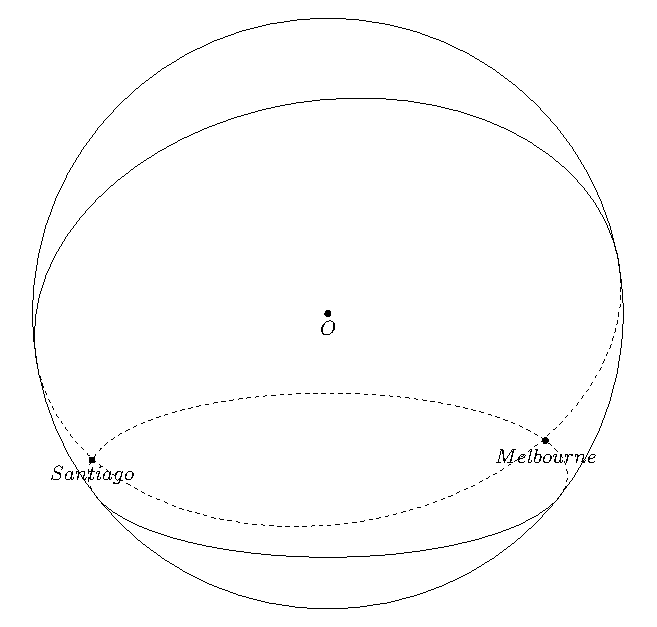
\includegraphics{Imagens/Tikz.pdf}
    \caption{Caminhos longitudinal e geodésico entre as cidades de Santiago e Melbourne.}
    \label{example}
\end{figure}

Note que esse exemplo ajuda a ilustrar o fato de que a geodésica é a curva de menor distância entre dois pontos em uma superfície, em especial na superfície esférica. Na prática, a geodésica pode ser utilizada como rota aérea e naval entre dois pontos distantes com o objetivo de diminuir o custo, tanto o temporal quanto o custo de combustível a ser utilizado na viagem.

\section{Rotações}
Seja $w = \alpha X_u + \beta X_v$. Queremos rotacionar esse vetor por um ângulo $\gamma$ nessa mesma base. Podemos fazer isso ortogonalizando e normalizando essa base, aplicando a matriz de rotação usual e depois obter os componentes da base original.

A ortogonalização da base é simplesmente 
\begin{equation*}
    \begin{array}{cc}
        \Tilde{X_u} = & X_u \\
        \Tilde{X_v} = & X_v - X_u \frac{\langle X_u, X_v \rangle}{\langle X_u, X_u \rangle} = X_v - X_u \frac{F}{E}
    \end{array}
\end{equation*}

O módulo ao quadrado do segundo vetor da base é 
\[\langle X_v, X_v \rangle - 2\frac{F}{E} \langle X_u, X_v \rangle + \frac{F^2}{E^2} \langle X_u, X_u \rangle = \]
\[ G - 2\frac{F^2}{E} + \frac{F^2}{E} = G - \frac{F^2}{E}\]

Então podemos escrever a base normalizada como 

\begin{equation*}
    \begin{array}{cc}
        \hat{X_u} = & \frac{X_u}{\sqrt{E}} \\
        \hat{X_v} = & \frac{X_v - X_u \frac{F}{E}}{\sqrt{G-\frac{F^2}{E}}}
    \end{array}
\end{equation*}

Como só precisamos de uma base ortogonal cujos vetores são de mesmo comprimento, podemos dividir ambos por $\sqrt{E}$

\begin{equation*}
\begin{array}{cc}
        X'_u = & \frac{X_u}{E} \\
        X'_v = & \frac{X_v - X_u \frac{F}{E}}{\sqrt{EG-F^2}}
    \end{array}
\end{equation*}

Podemos tomar $R = \sqrt{EG-F^2}$.

Agora podemos achar $w = \alpha' X'_u + \beta' X'_v$ substituindo.

\[w = \alpha' \frac{X_u}{E} + \beta' \frac{X_v}{R} - \beta' \frac{X_u F}{RE}\]

Na mesma base, os coeficientes de um vetor são únicos.

\begin{equation*}
    \begin{array}{cc}
        \alpha = & \frac{\alpha'}{E} - \frac{\beta' F}{RE}  \\
        \beta  = & \frac{\beta'}{R}
    \end{array}
\end{equation*}

\begin{equation*}
    \begin{array}{cc}
        \beta'  = & \beta R \\
        \alpha' = &\alpha E + \frac{\beta' F}{R} = \alpha E + \beta F
    \end{array}
\end{equation*}

O vetor rotacionado é
\[R_w = (\alpha' \text{cos} \gamma - \beta' \text{sin} \gamma)X'_u + (\alpha' \text{sin} \gamma + \beta' \text{cos} \gamma)X'_v\]
\[R_w = (\alpha' \text{cos} \gamma - \beta' \text{sin} \gamma)\frac{X_u}{E} + (\alpha' \text{sin} \gamma + \beta' \text{cos} \gamma)\frac{X_v - X_u\frac{F}{E}}{R}\]

\[R_w = \left( \alpha' \text{cos} \gamma - \beta' \text{sin} \gamma - (\alpha' \text{sin} \gamma + \beta' \text{cos} \gamma)\frac{F}{R} \right)\frac{X_u}{E} + \left( \alpha' \text{sin} \gamma + \beta' \text{cos} \gamma \right)\frac{X_v}{R}\]

\[R_w = \left( \alpha E \text{cos} \gamma - ( \frac{\beta R^2}{R} + \frac{\alpha EF}{R} + \frac{\beta F^2}{R})\text{sin} \gamma \right)\frac{X_u}{E} + \left( \alpha' \text{sin} \gamma + \beta' \text{cos} \gamma \right)\frac{X_v}{R}\]

\[R_w = \left( \alpha E \text{cos} \gamma - ( \frac{\beta EG}{R} + \frac{\alpha EF}{R})\text{sin} \gamma \right)\frac{X_u}{E} + \left( \alpha' \text{sin} \gamma + \beta' \text{cos} \gamma \right)\frac{X_v}{R}\]

\[R_w = \left( \alpha \text{cos} \gamma - \frac{\beta G + \alpha F}{R}\text{sin} \gamma \right)X_u + \left( \alpha' \text{sin} \gamma + \beta' \text{cos} \gamma \right)\frac{X_v}{R}\]

\[R_w = \left( \alpha \text{cos} \gamma - \frac{\alpha F + \beta G}{R}\text{sin} \gamma \right)X_u + \left( \frac{\alpha E + \beta F}{R} \text{sin} \gamma + \beta \text{cos} \gamma \right)X_v\]

\section{Aplicação computacional}
A nossa aplicação da equação geodésica é um programa gráfico 3d interativo que exibe uma superfície parametrizada dada pelo usuário. O usuário pode interagir com a câmera e com um ponto que pode se mover sobre a superfície. O ponto pode se mover nas direções das coordenadas ou na direção geodésica. É possível traçar o caminho andado pelo ponto ao se mover por geodésicos.

O programa não é simples, e por isso é dividido em partes: leitura de superfícies, computação simbólica, compilação de expressões, e um ambiente interativo que usa o método de Euler para encontrar geodésicos.

\subsection{Leitura de Superfícies}
Essa parte consiste em ler uma parametrização dada pelo usuário (em forma de texto) e interpretá-la para ser usada na computação simbólica. A expressão deve ser da forma \texttt{( x, y, z ) [min\_u, max\_u] [min\_v, max\_v] }, onde as expressões $x$, $y$ e $z$ são funções de $u$ e $v$. Os números $min\_u$, $max\_u$, $min\_v$ e $max\_v$ definem o domínio da aplicação em forma de retângulo.

A gramática dessas expressões é flexível. Ela inclui:
\begin{itemize}
    \item exponenciação: \texttt{u\textasciicircum 3}
    \item multiplicação por justaposição: \texttt{3u} é \texttt{3 * u}
    \item aplicação de funções sem parênteses: \texttt{cos u} é \texttt{cos(u)}
    
    Obs: o argumento da função pode ser (gramaticalmente) uma constante/número, uma variável, outra aplicação ou uma expressão entre parênteses.
    
    \item variáveis predefinidas: \texttt{u} e \texttt{v}
    \item constantes predefinidas: \texttt{pi} e \texttt{e}
    \item funções predefinidas: \texttt{sin}, \texttt{cos}, \texttt{tan}, \texttt{arcsin}, \texttt{arccos}, \texttt{arctan}, \texttt{exp}, \texttt{log} e \texttt{sqrt}
\end{itemize}

O texto é interpretado dessa forma e é gerado árvores sintáticas que representam as expressões dadas em texto pelo usuário. Essa forma é muito mais fácil de processar nos estágios seguintes.

\subsection{Computação simbólica}
É necessário computar várias derivadas para se chegar na equação geodésica. Para isso, o programa é capaz de derivar uma expressão simbolicamente, em relação a \texttt{u} ou \texttt{v}. Como as expressões são árvores sintáticas, a derivação pode ser feita recursivamente. Dependendo do tipo de expressão, uma regra de derivação específica é usada. Todos os tipos de expressão possuem uma regra de derivação, então qualquer expressão pode ser derivada. Esse processo de derivação é bastante verboso, fazendo a expressão final ter bastante redundâncias. Nosso programa não é capaz de simplificar essas redundâncias, então essas expressões não são viáveis de se calcular (para \texttt{u} e \texttt{v} dados) devido ao seu tempo de execução.

\subsection{Compilação de expressões}
Como dito, as expressões possuem redundâncias que as fazem ser muito mais lentas de se efetuar. Além disso, os \textit{overheads} da navegação pela árvore sintática também contribuem bastante para o tempo de execução. 

Para resolver esses dois problemas, a nossa solução foi uma só. Convertemos as expressões sintáticas novamente para a forma textual, mas dessa vez em forma de um programa em C++. Cada função relevante é convertido numa função C++ que calcula o valor dados \texttt{u} e \texttt{v}. Um compilador moderno é muito ágil em simplificar as expressões geradas pela derivação. Além disso, o cálculo dessas funções estarão na forma de código de máquina, fazendo seus cálculos serem inúmeras vezes mais rápidos. O código compilado é então carregado pelo nosso programa e as funções são encontradas e prontas para o uso.

O compilador também é extremamente rápido no seu trabalho. A esfera 
\[\left( \frac{1}{\sqrt{1+u^2+v^2}}, \frac{u}{\sqrt{1+u^2+v^2}}, \frac{v}{\sqrt{1+u^2+v^2}} \right)\]
gera um código de 15000 linhas. Mesmo assim, o compilador faz seu trabalho em menos de 1 segundo. 

\subsection{Ambiente interativo}
O ambiente interativo é construído usando OpenGL e C++. Para desenhar a superfície, o domínio da parametrização é cortado em vários retângulos, formando uma malha de pontos $uv$. O programa então gera uma amostra das imagens da malha $uv$, usando uma das funções compiladas. Uma vez gerada essa amostra, desenhar a superfície é mais rápida, pois os pontos já são conhecidos, basta desenhas os quadriláteros correspondentes.

O programa interage com o usuário através de um ponto sobre a superfície. Esse ponto pode ser movido nas direções das coordenadas ou em direções geodésicas, com direção inicial mutável. O programa também desenha os vetores da base, apontando para as linhas das coordenadas. Além disso, também desenha o vetor que define a direção para se andar em geodésicas.

O programa também pode fazer um traço do caminho percorrido pelo ponto, mas somente para caminhos geodésicos, e não para caminhos de coordenadas.

O usuário pode configurar a exibição da superfície, como número de pontos na amostra e visão grade das coordenadas. Além disso, é possível navegar com a câmera global. O usuário pode alterar entre visão global e visão local, cuja câmera fica grudada no ponto da superfície.

\begin{figure}
    \centering
    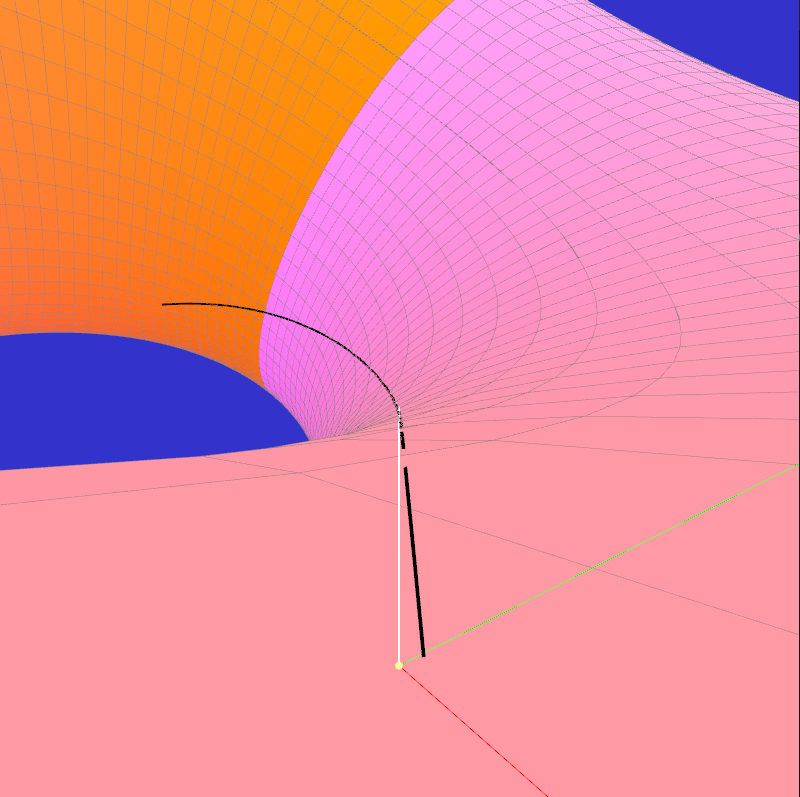
\includegraphics[scale = 0.5]{Imagens/torus.png}
    \caption{Curva geodésica num Toroide}
    \label{torus}
\end{figure}

\section{Conclusão}

Nesse trabalho introduzimos as geodésicas, com sua definição e demonstração de algumas de suas propriedades, incluindo a propriedade que diz respeito a geodésica ser a curva de menor caminho entre dois pontos em uma superfície. Além disso, viu-se um exemplo de geodésica que pode ser aplicado no dia a dia por empresas aéreas e navais, com o cálculo da geodésica em uma esfera, bem como o exemplo real da distância entre Santiago e Melbourne.

Também foi apresentado um programa em C++ com o intuito de ilustrar visualmente as geodésicas em algumas superfícies espaciais, possibilitando, inclusive, caminhar sobre as superfícies.

\newpage
\begin{thebibliography}{9}

\bibitem{wiki} Great Circle Distance. \textit{Wikipedia}. \url{https://en.wikipedia.org/wiki/Great-circle_distance}.

\bibitem{pixabay} Terra Verde Globo. \textit{Pixabay}.

\bibitem{folha} TEDESCO, L. A. del. (2017). Latam inaugura voo direto de 15 horas entre Chile e Austrália. \textit{Folha de S.Paulo}. \url{https://www1.folha.uol.com.br/turismo/2017/10/1925090-latam-inaugura-voo-direto-de-15-horas-entre-chile-e-australia.shtml}.

\bibitem{nunes} NUNES, B. (2010). Geometria Diferencial de Superfícies e o Teorema de Gauss-Bonnet. \textit{UFSC}. doi: \url{http://mtm.ufsc.br/~ebatista/Orientacoes_arquivos/tcc_bruna_certo.pdf}.

\bibitem{lima} LIMA, R. F. de (2016). Introdução à Geometria Diferencial. \textit{SBM}.

\bibitem{bruxel} BRUXEL, D. A. (2018). Um Estudo sobre Curvas Geodésicas. \textit{UFFS}. doi: \url{https://rd.uffs.edu.br/bitstream/prefix/2089/1/BRUXEL.pdf}.

\bibitem{matos} MATOS, A. C. de A. (2016). Geodésicas: Suas Equações e Algumas Aplicações. \textit{UEFS}. doi: \url{http://profmat.uefs.br/arquivos/File/ARIANA_CORDEIRO_DE_AMORIM_MATOS.pdf}.

\bibitem{fenn} FENN, R. (2007). Geometry. \textit{Springer}.

\bibitem{github} Grundmann, C.; Michels, I. P. (2021). \url{https://github.com/IgorMichels/Curves_and_surfaces}.

\end{thebibliography}

\end{document}